\chapter{Results}
Here we list the evaluation scores, and further guides we use for planning our next steps, available at the time of writing.

\section{Fully Convolutional Network}
Our overall impression with convolutional networks is that, they are slowly training, even high capacity networks are unable to achieve satisfactory score on training set~\ref{fig:convnet-overall}. For this reason, we aimed first to use an architecture, that is capable to over-fit on the train data, so we could fine-tune the training by enforcing the regularization settings.
\paragraph{MLP problem.}
A strange result is that by adding MLP block before the classifier, the performance was drastically reduced, and soon the training collapsed.
The models were biased towards only choosing a single class.
Excellent example for this behavior can be seen on Figure \ref{fig:convnet-bad}, where models with MLP built in oscillate around the same performance throughout an \textit{epoch}. (epoch: a set of training steps which includes every entry from the training set.)
We can also check out the confusion matrix of these models
on Figure \ref{fig:bad-conf-op}, also the histogram of the model parameters reveals, that the network is strongly biased towards choosing one specific class independently from its input in Figure \ref{fig:hist-op}.

\begin{figure}[h]
  \centering
  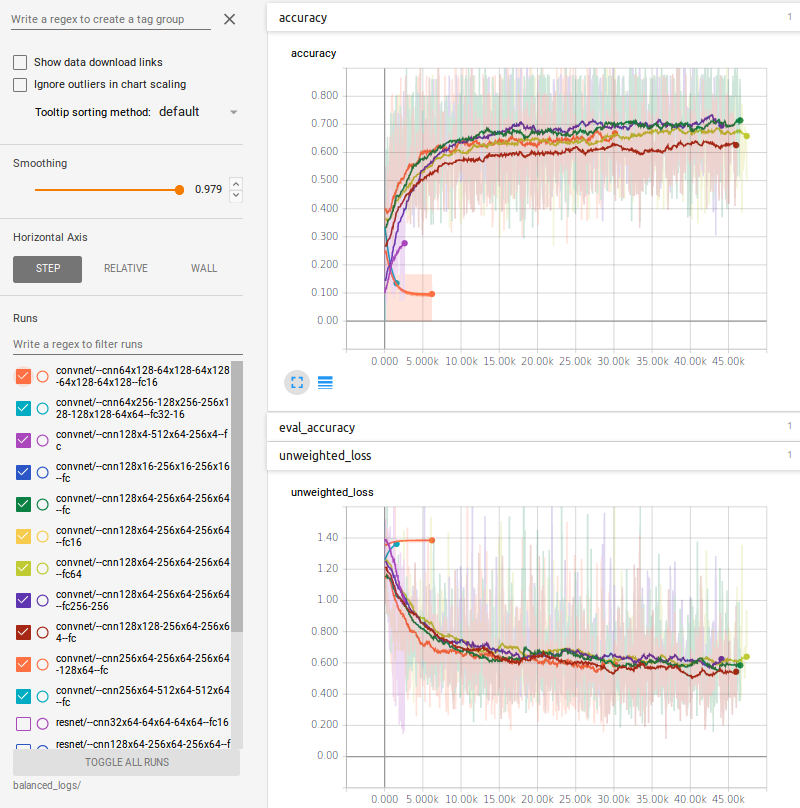
\includegraphics[width=\textwidth]{convnet-overall}
  \caption{Overall performance of the FCN approaches plotted in TensorBoard. Top: Accuracy derived from the confusion operator. Bottom: Unweighted loss during training}
  \label{fig:convnet-overall}
\end{figure}

\begin{figure}
  \centering
  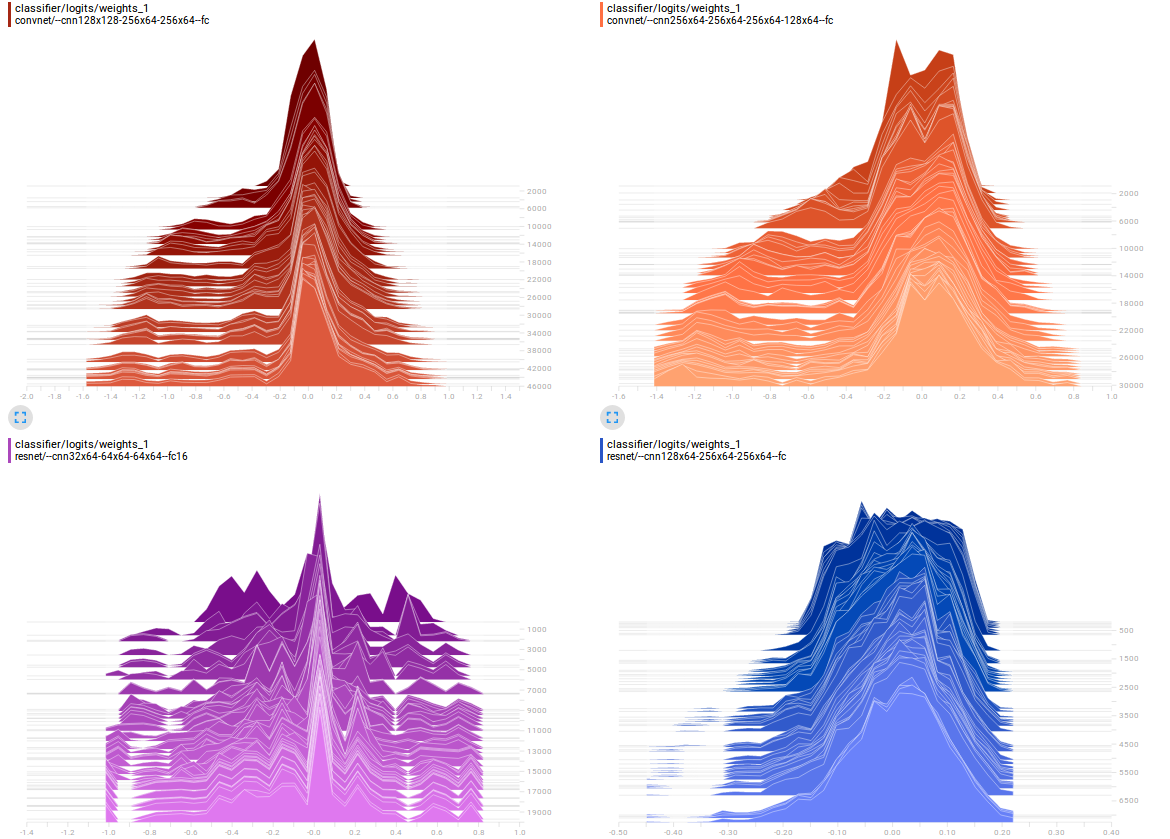
\includegraphics[width=\textwidth]{hist}
  \caption{Weight distribution of the classifier (last) layer through training. Note that networks with small variance, and local edgy peaks are more likely to fall into a local minimum of the parameter space --- where choosing the same class no matter what is the input is too stable state for the network to learn any further features.}
  \label{fig:hist-op}
\end{figure}

\begin{figure}
  \centering
  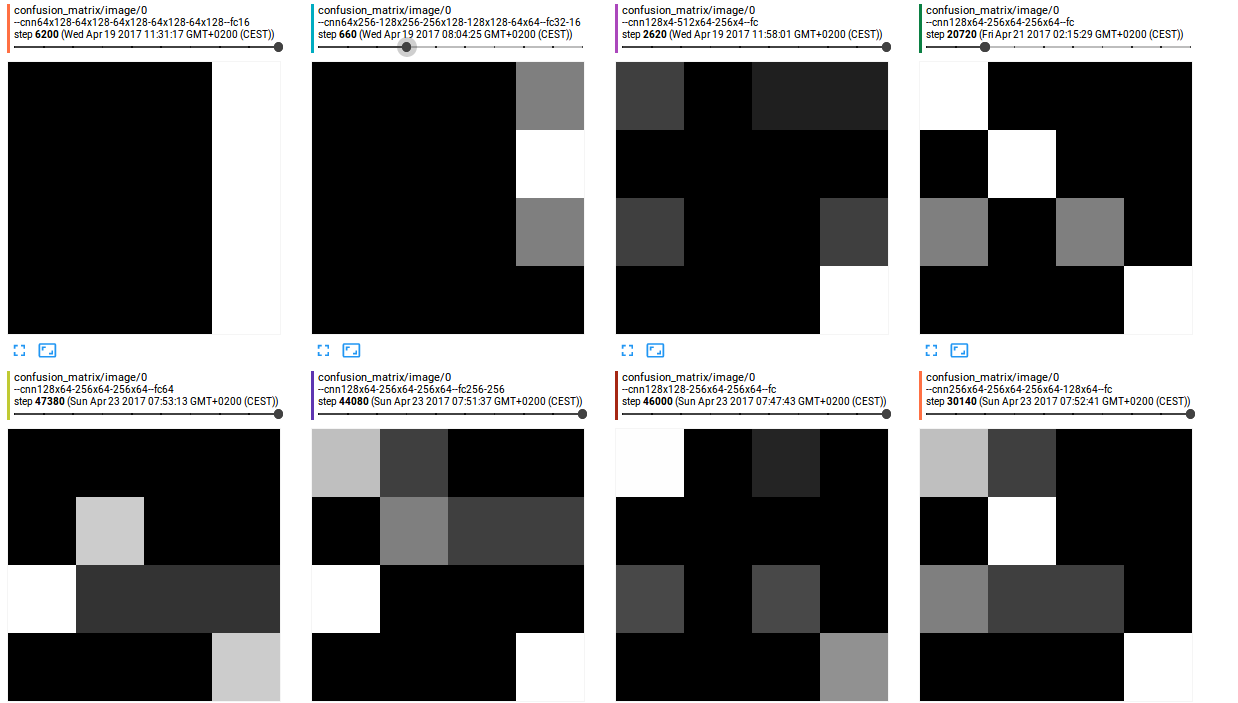
\includegraphics[width=\textwidth]{conf-op}
  \caption{Models are monitored through the training process: during weight updates a small subset of unseen entries is inferred, and compared to the ground truth labels. In these \textit{confusion matrices} the row sum represents a histogram of the labels, while the column sum would represent the histogram of the network's choice. Their intersection results in the talkative heat maps. Notice that those models whose confusion matrix is mainly diagonal is performing well, and those networks which have been collapsed gives a matrix where only a single column can be seen (i.e.~first row, the two rightmost matrix).}
  \label{fig:conf-op}
\end{figure}

\section{Residual Network}
Our next choice were deep residual networks.
With this model, we could achieve better training and evaluation scores.
The exclusion of the MLP block had to be made when using ResNets also, because the same behavior occurred when we applied hidden layers between feature extractors and the classifier layer.

\begin{figure}[h]
  \centering
  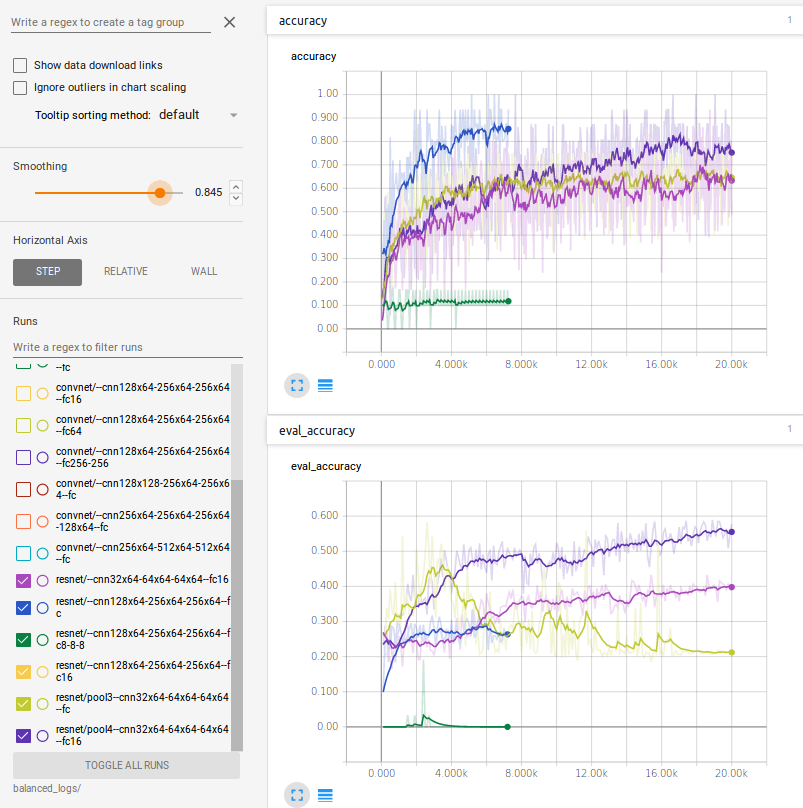
\includegraphics[width=\textwidth]{resnet-overall}
  \caption{Overall performance of the ResNet approaches plotted in TensorBoard. It is worth to mention that the network represented by the green curve is using the same hyper-parameters as the network with the highest train performance (blue), still because of the MLP block it fails to learn a generalized representation. Another important feature is that the network represented by the blue line performs way better on the training set, still fails on the evaluation set. This is the classical example of an over-fitted model. Top: Accuracy on the training set. Bottom: Accuracy on the evaluation set.}
  \label{fig:resnet-overall}
\end{figure}
